Уменьшения ошибки измерения можно добиться, в основном, следующими методами:

\begin{enumerate}
    \item Two Way Time Transfer.
    \item Code Modulus Synchronization.
    \item Frequency Diverse Range Estimation.
\end{enumerate}

\subsubsection{Two Way Time Transfer}

Метод <<Two Way Time Transfer>> (TWTT) --- метод, позволяющий устранить рассогласование начала отсчёта тактовой частоты двух устройств. Этот метод позволяет игнорировать смещение начала отсчёта первого устройства по отношению ко второму $\delta t$. Алгоритм работы TWTT показан на рисунке~\ref{fig:twttmethod}.

\begin{figure}[ht]
    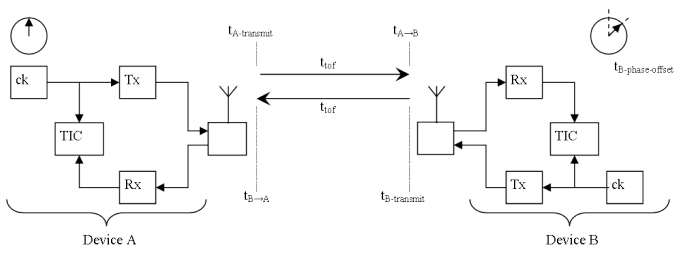
\includegraphics[width=1\linewidth]{Figures/twttmethod.png}
    \caption{Алгоритм работы метода Two-way Time Transfer}
    \label{fig:twttmethod}
\end{figure}

Метод заключается в следующем: оба устройства (А и Б) участвуют в измерении времени используя локальный (собственный) тактовый генератор. Если устройство А отправляет посылку в момент времени $t_{sA}$, устройство Б принимает посылку в момент времени $t_{rB}$, устройство Б отправляет посылку в момент времени $t_{sB}$ и устройство А принимает посылку в момент времени $t_{rA}$, причём $t_{sA} < t_{rB} < t_{sB} < t_{rA}$, тогда устройство A измерит время $t_A = t_{rA} - t_{sA}$, а устройство Б измерит время $t_B = t_{sB} - t_{rB}$. \textit{Time of Flight}, TOF, $\tau$ может быть выражена используя эти два времени следующим образом (формула~\eqref{eq:twtt}):

\begin{equation}
    \label{eq:twtt}
    \tau = \frac{t_A - t_B}{2}.
\end{equation}

В общем случае, можно представить метод Two-way Time Transfer следующими выражениями~\cite{tof:ranging}:

\begin{equation}
    t_{A \to B} = t_{A - transmit} + t_{TOF} + t_{B - offset}
\end{equation}

\begin{equation}
    t_{B \to A} = t_{B - transmit} + t_{TOF} - t_{B - offset}
\end{equation}

Тогда,

\begin{equation}
    t_{TOF} = \frac{1}{2}[(t_{A \to B} + t_{B \to A}) - (t_{A - transmit} + t_{B - transmit})]
\end{equation}

\begin{equation}
    t_{offset} = \frac{1}{2}[(t_{A \to B} - t_{B \to A}) - (t_{A - transmit} - t_{B - transmit})]
\end{equation}

%\subsubsection{Code Modulus Synchronization}

%Empty.

%\subsubsection{Frequency Diverse Range Estimation}

%Empty.
